\documentclass[conference,a4paper,10pt, oneside,final]{tfmpd}
%\usepackage[latin1]{inputenc}   % caracteres especiales (acentos, eñes)
%\usepackage[spanish]{babel}     % varias definiciones para el español
\usepackage[utf8x]{inputenc}
\usepackage{graphicx}           % inserción de graficos
\usepackage{float} %paquete para que ponga las imagenees donde yo quiero, no donde quiere el muy hdp de latex
%la posición de la imagen, con H (mayúscula!!)

\usepackage{amssymb}
\usepackage{amsfonts}
\usepackage{amsmath}

\begin{document}

\title{Técnicas de Esteganografía en señales de audio.}

\author{Darío A. Villarreal,
        Esteban J. Zeller y
        Matías A. Eberhardt\\
\textit{Trabajo Práctico Final de Procesamiento Digital de Señales, II-FICH-UNL.}}

\markboth{Trabajo Práctico Final de Procesamiento Digital de Señales}{}

\maketitle

\begin{abstract}
En este trabajo haremos una breve clasificación de las técnicas de esteganografía existentes y su diferenciación con otras disciplinas de protección de datos digitales. Luego decribiremos e implementaremos dos de dichas técnicas: Modificación del Bit Menos Significativo (LSB, Least Significant Bit) en el dominio temporal y en el dominio frecuencial se ocultará la información en los coeficientes de la Tranformada Wavelet Discreta. Finalmente evaluaremos los resultados obtenidos mediante técnicas objetivas y subjetivas.
\end{abstract}

\begin{keywords}
esteganografía, data hidding, watermarking, seguridad de la información
\end{keywords}

\section{Introducción}
\PARstart{L}{a} esteganografía es una disciplina que se dedica a ocultar mensajes u objetos dentro de otros llamados portadores de modo que su inclusión pase desapercibida. Básicamente explota las limitaciones de la percepción humana, ya que nuestros sentidos presentan límites para percibir pequeñas alteraciones en las señales.
Pese a que es usada desde la antigüedad, esta disciplina ha suscitado mucho interés en las últimas décadas, especialmente en el área de la seguridad de la información dado el crecimiento del uso de la red de comunicaciones. La gran cantidad de información digital que circula en ella ha hecho que profesionales de la industria e investigadores prestaran especial atención en la seguridad de los datos digitales, siendo las principales disciplinas la criptografía, esteganografía y watermarking. 

\begin{figure}[h!]
 \centering
 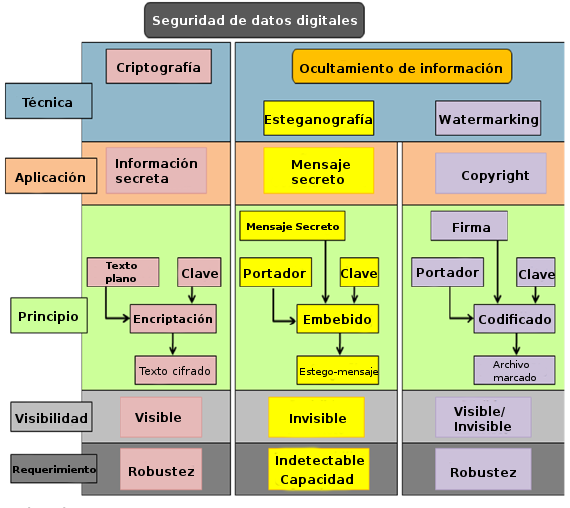
\includegraphics[keepaspectratio=true, width=240 px]{./cuadro.png}
 % cuadro.png: 0x0 pixel, 300dpi, 0.00x0.00 cm, bb=
 \caption{Disciplinas de segudidad de datos digitales}
 \label{fig: Disciplinas de segudidad de datos digitales}
\end{figure}

La criptografía busca evitar que cierta información pueda ser leída por personas sin autorización, por lo que su principal requerimiento es la robustez ante los intentos de descifrado. El watermarking busca dejar una huella (visible o invisible) identificable y robusta ante ataques y compresión en imágenes, audio y vídeo. Para el diseño de técnicas esteganográficas los tres parámetros a tener en cuenta son la capacidad de ocultamiento de información, la imperceptibilidad y la robustez, pero es imposible obtenerlos al mismo tiempo. Estos parámetros se grafican como los vértices de un triángulo equilátero, donde acercarse al cumplimiento de uno es alejarse de los otros. Por ejemplo, los métodos con más capacidad son sensibles al ruido y la compresión, mientras que los métodos robustos presentan una baja capacidad de ocultamiento de información.

Entre las aplicaciones prácticas de la esteganografía digital se encuentran la conunicación encubierta, inclusión de copyright en archivos multimedia, ocultar ejecutables para obtener datos de uso o acceso a un equipo remoto, entre otros.

En este trabajo repasaremos brevemente las principales técnicas de esteganografía digital en archivos de audio, luego implementaremos dos de ellas y finalmente analizaremos los resultados obtenidos.

\section{Métodos esteganográficos \cite{journals/ejasmp/DjebbarA12}}

\subsection{En el dominio del tiempo}
Los métodos en el dominio del tiempo se caracterizan por simplicidad, alta capacidad e imperceptibilidad.
\begin{itemize}
 \item Bit menos significativo (LSB)
 \begin{itemize}
 \item Los bits menos significativos de cada muestra son reemplazados por la información a codificar
 \item Ventajas: Simples de codificar. Alta capacidad de embebido
 \item Desventajas: Fácil de extraer y destruir
 \item Tasa de ocultado de información: 16kbps
 \end{itemize}
 \item Echo hidding
  \begin{itemize}
 \item Se incorporan ecos en el audio portador por convolución para embeber el mensaje.
 \item Ventaja: Resistende a algoritmos de compresión con pérdida
 \item Desventaja: Baja capacidad y seguridad.
 \item Tasa de ocultado de información: 50bps
 \end{itemize}
 \item Intérvalos de silencio
  \begin{itemize}
 \item Se usa el número de muestras de los intervalos de silencio para esconder información.
 \item Ventaja: Resistende a algoritmos de compresión con pérdida
 \item Desventaja: Baja capacidad.
 \item Tasa de ocultado de información: 64bps
 \end{itemize}
\end{itemize}

\subsection{En el dominio de la frecuencia}
\begin{itemize}
 \item Magnitud del espectro
   \begin{itemize}
 \item Usa las bandas de frecuencia para ocultar información
 \item Ventaja: Alta capacidad, 
 \item Desventaja: Baja robustez a manipulaciones simples de audio
 \item Tasa de ocultado de información: 20kbps
 \end{itemize}
 \item Inserción de tono
 \begin{itemize}
 \item La información se codifica insertando tonos a frecuencias seleccionadas
 \item Ventajas: Imperceptibilidad e indetectabilidad del mensaje embebido.
 \item Desventaja: Baja capacidad. Los tonos son fácilmente detectables si se sospecha que hay información oculta, sería fácil reemplazar la información embebida.
 \item Tasa de ocultado de información: 250bps
 \end{itemize}
 \item Espectro de fase
 \begin{itemize}
 \item Se modula la fase de la señal portadora.
 \item Ventajas: Es robusto frente a manupulaciones del audio. Para recuperar la información se necesita la señal original.
 \item Desventaja: Baja capacidad.
 \item Tasa de ocultado de información: 333bps
 \end{itemize}
 \item Dispersión en el espectro (spread spectrum)
  \begin{itemize}
 \item Se dispersa la información a ocultar en todo el espectro de frecuencias.
 \item Ventajas: Su alta redundancia la hace muy robusta ante distorsiones de la señal.
 \item Desventaja: Vulnerable al modificado de la escala temporal de la señal
 \item Tasa de ocultado de información: 20bps
 \end{itemize}
 \item Dominio Cepstral
   \begin{itemize}
 \item Se modifican los coeficientes cepstrales para embeber la señal.
 \item Ventajas: Robusto ante operaciones de procesamiento de señales.
 \item Desventaja: Incorpora distorsiones perceptibles.
 \item Tasa de ocultado de información: 54bps
 \end{itemize}
 \item Wavelets
    \begin{itemize}
 \item Se modifican los coeficientes wavelets para codificar la información.
 \item Ventajas: Alta capacidad de embebido.
 \item Desventaja: Recuperación con pérdida de información.
 \item Tasa de ocultado de información: 70kbps
 \end{itemize}
\end{itemize}


\subsection{En la codificación/decodificación}
\begin{itemize}
 \item Modificación de los codebooks
     \begin{itemize}
 \item Se modifican los parámetros de los diccionarios de codificado y decodificado.
 \item Ventaja: Robusto
 \item Desventaja: Baja capacidad de embebido.
 \item Tasa de ocultado de información: 2kbps
 \end{itemize}
 \item Ocultamiento en el flujo de bits
      \begin{itemize}
 \item Se le modifican los bits menos significativos del flujo de bits resultantes del proceso de codificado.
 \item Ventaja: Robusto
 \item Desventaja: Baja capacidad de embebido.
 \item Tasa de ocultado de información: 1.6kbps
 \end{itemize}
\end{itemize}

\section{Implementación en el dominio temporal: Bit menos significativo (LSB)}
La modificación LSB es una de las técnica de esteganografía más simple que provee una alta capacidad. Esta ténica consiste en ocultar el mensaje en el o los bits menos significativos de la muestras de audio.
Incrementando el numero de bits a modificar se induce mas ruido, si dicho audio supera un determinado umbral y es percibido, la técnica falla. Por lo tanto usando mas LSBs se incrementa la capacidad pero se pierde transparencia.

La tecnica de LSB es vulnerable al estegoanálisis. Realizando un analisis de la señal se podria detectar facilmente el mensaje secreto.
Se proponen dos variantes a la técnica de LSB que la mejoran:

\subsubsection{Seleccion de Bit}

En esta tecnica utiliza los primeros dos bits mas significativos de cada muestra para decidir cual bit de la misma muestra va a contener el bit del mensaje secreto. El mensaje secreto se ocultara en uno de los primeros tres LSBs de cada muestra.

Si los primeros dos MSBs de la muestra son iguales a $00$, el tercer LSB sera reemplazado con un bit del mensaje secreto. Si los primeros dos MSBs de la muestra son iguales a $01$, el segundo LSB sera reemplazado con un bit del mensaje secreto y si los dos primeros MSBs son $10$ o $11$, el primer bit sera reemplazado por un bit del mensaje secreto.
De esta manera se introduce una aleatoriedad en la seleccion de los bits donde se ocultara el mensaje.

\subsubsection{Seleccion de Muestra}
Otra manera de agregar aleatoreidad es usar solo algunas muestras de la señal. Esto es controlado por los primeros tres MSBs de una muestra. Es decir si "i" es la muestra actual, los primeros tres MSBs de i determinaran el numero de muestras salteadas entre dos bits consecutivos del mensaje secreto. Por ejemplo si los primeros tres MSBs de la primera muestra (i=1) son iguales a 010, entonces la proxima muestra que contendra el siguiente bit del mensaje secreto sera i+3=4. Luego la proxima muestra estara determinada por los tres primeros MSBS de la muestra 4 y asi sucesivamente. Este método brinda una mayor aleatoreidad que el anterior pero decrementa la capacidad.


\section{Implementación en el dominio frecuencial}
Este método se basa en embeber la información en los bits menos significativos de los coeficientes enteros de la transformada wavelet discreta. 
En este trabajo utilizamos la familia de wavelets Haar por ser las mas simples, rápidas y eficientes en lo que al cálculo se refiere y la transformada LWT (Lifting Wavelet Transform) para obtener coeficientes enteros. Luego, para mejorar la imperceptibilidad se emplearon umbrales calculados sobre el tamaño del coeficiente embebiendo menos bits en coeficientes pequeños y evitando embeber información en los tramos silenciosos del archivo de audio.

\scriptsize{
$$
Th_i= \left\lbrace 
\begin{array}{ll}
 nbits - fijos -1 \quad si \quad C_i \geq 2^{nbits-1}\\
 \\
nbits - fijos -3 \quad si \quad 2^{nbits-1} \geq C_i \geq 2^{nbits-3} \\
\\
nbits - fijos -5 \quad si \quad 2^{nbits-3} \geq C_i \geq 2^{nbits-5} \\
\\
nbits - fijos -7 \quad si \quad 2^{nbits-5} \geq C_i \geq 2^{nbits-7} \\
\\
0 \qquad  \text{en otro caso.} 
\end{array}
\right.
$$
}

Donde $Th$ es el vector umbral que indica cuandos bits embeberemos en cada coeficiente, $C$ es el vector de coeficientes, $nbits$ es el tamaño en bits del coeficiente wavelet entero, $fijos$ son los MSBs que no se tocarán.

Presenta una alta imperceptbilidad y capacidad.

\section{Evaluación de resultados}
\subsection{PEAQ}
\begin{figure}[h!]
 \centering
 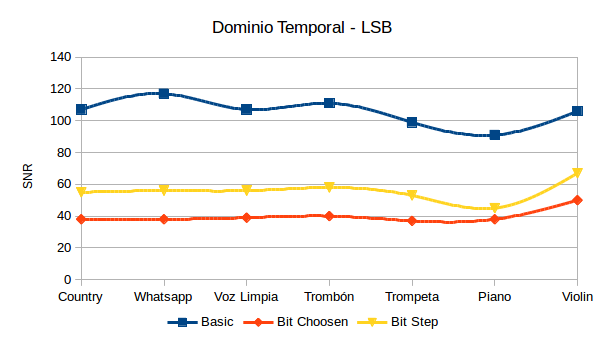
\includegraphics[keepaspectratio=true, width=240 px]{./graficos/dominio-temporal-lsb-snr.png}
 % dominio-temporal-lsb-snr.png: 0x0 pixel, 300dpi, 0.00x0.00 cm, bb=
 \caption{Leyenda}
 \label{fig: etiqueta}
\end{figure}

\begin{figure}[h!]
 \centering
 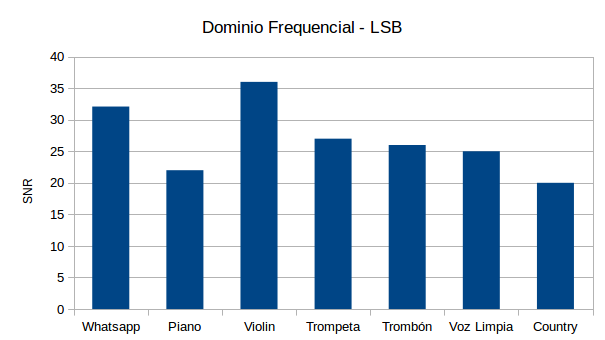
\includegraphics[keepaspectratio=true, width=240 px]{./graficos/dominio-frequencial-lsb-snr.png}
 % dominio-frequencial-lsb-snr.png: 0x0 pixel, 300dpi, 0.00x0.00 cm, bb=
 \caption{Leyenda}
 \label{fig: Etiqueta}
\end{figure}


\section{Conclusiones}

\nocite{*}
\bibliographystyle{tfmpd}
\bibliography{tfmpd}

\end{document}
